% ***********************************************************
% ******************* PHYSICS HEADER ************************
% ***********************************************************
% Version 2
\documentclass[11pt]{article} 
\usepackage{amsmath} % AMS Math Package
\usepackage{amsthm} % Theorem Formatting
\usepackage{amssymb}	% Math symbols such as \mathbb
\usepackage{graphicx} % Allows for eps images
\usepackage{multicol} % Allows for multiple columns
\usepackage[dvips,letterpaper,margin=1in,top=1in,bottom=1in]{geometry}
\renewcommand{\labelenumi}{(\alph{enumi})} % Use letters for enumerate
% \DeclareMathOperator{\Sample}{Sample}
\let\vaccent=\v % rename builtin command \v{} to \vaccent{}
\renewcommand{\v}[1]{\ensuremath{\mathbf{#1}}} % for vectors
\newcommand{\gv}[1]{\ensuremath{\mbox{\boldmath$ #1 $}}} 
% for vectors of Greek letters
\newcommand{\uv}[1]{\ensuremath{\mathbf{\hat{#1}}}} % for unit vector
\newcommand{\abs}[1]{\left| #1 \right|} % for absolute value
\newcommand{\avg}[1]{\left< #1 \right>} % for average
\let\underdot=\d % rename builtin command \d{} to \underdot{}
\renewcommand{\d}[2]{\frac{d #1}{d #2}} % for derivatives
\newcommand{\dd}[2]{\frac{d^2 #1}{d #2^2}} % for double derivatives
\newcommand{\pd}[2]{\frac{\partial #1}{\partial #2}} 
% for partial derivatives
\newcommand{\pdd}[2]{\frac{\partial^2 #1}{\partial #2^2}} 
% for double partial derivatives
\newcommand{\pdc}[3]{\left( \frac{\partial #1}{\partial #2}
 \right)_{#3}} % for thermodynamic partial derivatives
\newcommand{\ket}[1]{\left| #1 \right>} % for Dirac bras
\newcommand{\bra}[1]{\left< #1 \right|} % for Dirac kets
\newcommand{\braket}[2]{\left< #1 \vphantom{#2} \right|
 \left. #2 \vphantom{#1} \right>} % for Dirac brackets
\newcommand{\matrixel}[3]{\left< #1 \vphantom{#2#3} \right|
 #2 \left| #3 \vphantom{#1#2} \right>} % for Dirac matrix elements
\newcommand{\grad}[1]{\gv{\nabla} #1} % for gradient
\let\divsymb=\div % rename builtin command \div to \divsymb
\renewcommand{\div}[1]{\gv{\nabla} \cdot #1} % for divergence
\newcommand{\curl}[1]{\gv{\nabla} \times #1} % for curl
\let\baraccent=\= % rename builtin command \= to \baraccent
\renewcommand{\=}[1]{\stackrel{#1}{=}} % for putting numbers above =
\newtheorem{prop}{Proposition}
\newtheorem{thm}{Theorem}[section]
\newtheorem{lem}[thm]{Lemma}
\theoremstyle{definition}
\newtheorem{dfn}{Definition}
\theoremstyle{remark}
\newtheorem*{rmk}{Remark}

% ***********************************************************
% ********************** END HEADER *************************
% ***********************************************************

\usepackage{graphicx}
\bibliographystyle{plain}
\title{Percolation in Random Resistor Networks}
\author{Forrest Sheldon}
\date{\today}
\begin{document}
\maketitle

\section{Introduction}

Percolation deals with the properties of clusters created by some
probabilistic means. Generally, past a threshold an infinite cluster
will form that spans the lattice and we consider this a phase transition.
While the process that generates this cluster is simply stated, its properties
are quite rich, resisting analytic treatment and exhbiting complex phenomena
such as multifractal scaling. The marriage of conceptual simplicity and
complex behavior makes percolation a popular introduction to phase transitions,
and the generality of the model makes it applicable to a wide variety of physical
problems from superconductivity to forest fires.


This coverage aims to give an introduction to percolation theory with particular
attention to the problem as a conduction transition in a random resistor network.
We will follow our coverage of the Ising model, first introducing percolation and
giving brief attention to it's variants and correspondence to physical transitions.
Then we will
review exact solutions on simple lattices, namely in one dimension and the Bethe
lattice.  Next we will review mean field theory techniques away from the transition
and then scaling relations derivable from assumptions about the form of the
infinite cluster.  Finally, we will review applications of renormalization, and give
a summary of extensions to more complex examples.

\subsection{The Basic Percolation Problem}

Consider a finite cubic lattice where neighboring sites are not yet connected.
At every potential edge, place a bond with a probability, or \textbf{concentration}
$p$. As we increase this concentration from 0, at some point instantiations of the
lattice will contain clusters that connect from the top to the bottom and we say
the lattice \textbf{percolates}.  As the size of the lattice
increases, the point at which a percolating cluster forms becomes more sharply
defined and in the infinite limit we can define a critical concentration
$p_c$ beyond which an infinite cluster exists.

We may consider a similar problem where bonds are all occupied but \emph{sites}
are initially vacant.  Each site is occupied with a probability $p$ and clusters
are collections of occupied sites connected by bonds.  This defines the
\textbf{site percolation} as opposed to \textbf{bond percolation} mentioned previously.
Depending on the physical problem we are interested in, we may choose to frame
it in terms of sites or bonds but the results given by either will be closely
related.  Here we will focus on bond percolation with the intention of relating our
results to the random resistor network.  This coverage is adapted from
\cite{Stauffer1994} \cite{Christensen2002} which both cover site percolation.
Results here have been rederived for bond percolation following their arguments.

%==================================================================================
% IMPORTANT QUANTITIES AND EXPONENTS
%==================================================================================

\subsection{Important Quantities and Exponents}

We will make use of several quantities to characterize the lattice and it's transition.
Here we give a brief summary of each, important relations
involving them and their critical exponents:

\begin{enumerate}

\item[$p_c\quad$] The \textbf{percolation threshold} is the concentration at which an infinite cluster
will form on an infinite lattice.  While easily evaluated on the Bethe lattice, analytical
results resisted attempts for 20 years after the problem was initally posed.  As with
the critical temperature, it is nonuniversal and depends on the details of the lattice
structure.  Currently accepted values may be viewed in Table \ref{tab:perc_thresh}.

\begin{table}
  \centering
  \begin{tabular}{ | l | r | l | l | }
    \hline
    Lattice & Coord. \# & Site & Bond \\
    \hline \hline
    1d & 2 & 1 & 1 \\ \hline
    2d Honeycomb & 3 & 0.6962 & $1-2\sin{\pi/8}\approx 0.65271$ \\ \hline
    2d Square & 4 & 0.592746 & 1/2 \\ \hline
    2d Triangular & 6 & 1/2 & $2\sin{\pi/18}\approx 0.34729$ \\ \hline
    3d Diamond & 4 & 0.43 & 0.388 \\ \hline
    3d Simple cubic & 6 & 0.3116 & 0.2488 \\ \hline
    4d Hypercubic & 8 & 0.197 & 0.1601 \\ \hline
    5d Hypercubic & 10 & 0.141 & 0.1182 \\ \hline
    Bethe Lattice & z & $1 / (z-1)$ & $1 / (z-1)$ \\ \hline
  \end{tabular}
  \caption{Percolation thresholds for various lattices.  Note that within a dimension,
           the threshold decreases with increasing coordination number.  This is an
           abridged version of a table found in \cite{Christensen2002}.}
  \label{tab:perc_thresh}
\end{table}

\item[P(p)] The \textbf{strength} of the infinite cluster gives the probability that
an arbirary bond is connected to the infinite cluster.  As such, $P$ is 0 below
the percolation threshold and goes to 1 as $p\to 1$.  In most lattices, at $p_c$
$P$ increases continuously from 0 and so is analogous to our order parameter for a second
order phase transition.  This allows us to define the critical exponent $\beta$,
\[ P(p) \propto (p - p_c)^{\beta} \ \text{as}\ p\to p_c^+ \]

\item[$n_s(p)$] The \textbf{cluster number distribution} gives the average number of
clusters of size $s$ per lattice site (such that in a lattice of size $N$ there will be on
average $Nn_s(p)$ clusters of size $s$ at concentration $p$).  As all bonds must belong
to a cluster of some size, we have,
\begin{align*}
\sum_s sn_s(p) = p,&\quad p<p_c \\
\sum_s sn_s(p)+ P(p) = p,&\quad p>p_c \\
\end{align*}
 where the sum excludes the infinite cluster. This
quantity $sn_s(p)$ is somewhat
analogous to a Boltzman weight in that it gives us information on the probabilities of
certain configurations of the system.

\item[$s_\xi\quad$] We will find that the cluster number
distribution away from the percolation threshold, $n_s \propto \exp{(s/s_\xi)}$.
The scaling factor in the denominator is the \textbf{cutoff cluster size}.  This will
generally diverge at the percolation threshold allowing us to define the critical exponent
$\sigma$
\[ s_\xi \propto |p_c - p|^{-\frac{1}{\sigma}} \ \text{as}\ p\to p_c \]

\item[$S$\quad] The cluster number distribution allows us to calculate a \text{mean cluster
size} which we define as the average cluster size to which a given occupied bond belongs.
As the fraction of occupied bonds belonging to s clusters is
\(\frac{sn_s(p)N}{pN} = \frac{sn_s(p)}{\sum sn_s(p)}\) the average cluster size is
\[S(p) = \frac{\sum s^2 n_s(p)}{\sum s n_s(p)}\]
(Note that in this definition clusters are sampled by \emph{bond} biasing our selection
towards larger clusters.  We could similarly have defined an average cluster size in which
all clusters are sampled with equal probablity
\(S'(p) = \frac{\sum s n_s(p)}{\sum  n_s(p)}\) but we will find that our current definition
is more appropriate.) This is analogous to our susceptibility in thermal problems.

The mean cluster size will also diverge at the percolation threshold, allowing us to
define the critical exponent $\gamma$
\[ S \propto |p_c - p|^{-\gamma} \ \text{as}\ p\to p_c \]

\item[$g(r)$] The \textbf{correlation function} or \textbf{pair connectivity} is the
probability that a bond a distance $r$ away from an occupied site belongs to the same
cluster.  In analogy to the susceptibilty sum rule, we have a relation between the
correlation function and the mean cluster size,
\[\sum_{\vec{r}} g(\vec{r}) = S\]
which is our motivation for defining the average cluster size as we have.

\item[$\xi\quad$] The \textbf{correlation length} is the rms radius of a typical
cluster.  We can define it through the normalized correlation function
$\frac{g(r)}{S(p)}$ as,
\[\xi^2 = \frac{1}{S(p)}\sum_{\vec{r}}r^2 g(\vec{r}).\]
It will typically diverge at the percolation threshold,
allowing us to define the critical exponent $\nu$,
\[ \xi \propto |p_c - p|^{-\nu} \ \text{as}\ p\to p_c \]
\end{enumerate}

%==================================================================================
% EXACT SOLUTIONS
%==================================================================================

\section{Exact Solutions}

In this section we will calculate the preceding quantities in two scenarios in which they
may be evaluated exactly: the one dimensional chain and the Bethe Lattice.  Again
similar coverages for site percolation (which is identical to bond percolation in 1d)
may be found in \cite{Stauffer1994} \cite{Christensen2002}

\subsection{One-Dimension}

On an infinite lattice, any unoccupied bond will break the infinite cluster and thus
we can only have percolation at $p_c = 1$ (in analogy with the 1d Ising model).  The
strength $P(p)$ is thus zero for $p<1$ and jumps discontinuously to $1$ at percolation.

To find the cluster number distribution, we note that the probability for a cluster
of size $s$ to lie at any given position is $p^s(1-p)^2$.  As the number of possible
locations for such a cluster is equal to the number of bonds we have (from the linearity
of the expectation) that the expected number of such clusters \emph{per bond} is
\[n_s(p) = p^s(1-p)^2\]
As a check, we can evaluate,
\begin{align*}
\sum_s sn_s(p) &= \sum_s sp^s(1-p)^2 \\
 &= (1-p)^2 (p\d{}{p})\sum_s p^s \\
 &= p\frac{(1-p)^2}{(1-p)^2} = p
\end{align*}
We may write this
quantity as,
\[n_s(p) = (p_c - p)^2\exp{(-s/s_\xi)}, \quad s_\xi = -\frac{1}{\ln{p}}\]
and obtain the cutoff cluster size.  We thus have
\[s_\xi = -\frac{1}{\ln(1 - (p_c - p))}\propto |p_c - p|^{-1}\]
yielding the critical exponent $\sigma=1$.

To evaluate the average cluster size, we proceed as with our previous check on
the cluster number distribution to obtain,
\[S = \frac{\sum_s s^2n_s(p)}{\sum_s sn_s(p)} = \frac{1+p}{1-p}\]
and we can immediately identify $\gamma=1$.

In order for two bonds separated by a distance $r$ to be connected, all
bonds between them must be connected and thus \(g(r) = p^r$.  We can confirm the susceptibility sum rule noting that the sum over
$\vec{r}$ breaks into a contribution from $r=0$ and two from bonds to the left and
right.
\[\sum_{\vec{r}}g(r) = 1 + 2\sum_{r=1,2..} p^r = 
1 + 2p\sum_{s=0,1,2..} p^s= \frac{1+p}{1-p} = S.\]

Lastly, to obtain the correlation length, we evaluate
\begin{align*}
\xi^2 =& \frac{1-p}{1+p}\:\sum_{\vec{r}}r^2p^r \\
=& \frac{1-p}{1+p}\left(p\d{}{p}\right)^2 2\sum_{r=1,2...}p^r \\
=& \frac{2p}{(1-p)^2}
\end{align*}
and we find $\nu = 1$.

\subsection{Bethe Lattice/Mean-Field Solution}

The Bethe lattice is an infinite tree (read no loops) in which each site has
$z$ nearest neighbors.  If $z=2$ we regain the 1d chain. The Bethe lattice is 
so named for the Bethe Peierls
approximation whose results are exact when applied to the Bethe lattice.
Readers interested in its history and breadth of application in physics
can consult Thorpe's charming and seemingly obscure coverage in \cite{Thorpe1982}.

Considering entering a site through an occupied bond, we expect that the lattice will
percolate when the expected number of bonds continuing onward is 1.  This yields the
correct percolation threshold of $p_c = \frac{1}{z-1}$ which may be established
through more rigorous and complex methods \cite{Fisher1961}.

In order to obtain the strength of the infinite cluster, we consider a arbitrary
bond in the lattice.  In order for this bond to be connected to the infinite
cluster, it must be occupied and at least one neighboring bond must be connected
to the cluster.  This begs us to introduce the probability $Q$ that a given neighboring
bond is not part of the infinite cluster.  The structure of the Bethe lattice allows us
to obtain a self-consistent equation for the probability $Q$.  If a bond does not
connect to infinity, it must be either unoccupied, or occupied and none of its
neighboring bonds connects to infinity, $Q = (1-p) + pQ^{z-1}$.  Aside from
perturbatively, I am not sure how to solve this for arbitrary $z$ (If anyone
reading this knows how, I would appreciate an e-mail. While I know that an arbitrary
higher degree polynomial is not analyticaly soluble, I am not so pessimistic about
the depressed form here.)  We will examine the situation in the
simpler regime where $z=3$.  Here we can solve, $pQ^2 - Q + (1-p) = 0$ giving the
two solutions $Q=1, \frac{1-p}{p}$. The probability that an arbitrary bond is both
occupied and connects to the infinite cluster is then,
\[P(p) = p(1-Q^4) = \frac{p^4-(1-p)^4}{p^3}.\]
Evaluation at the percolation threshold yields $P(p_c) = 0$ as expected and
$P'(p_c)>0$ which requires $\beta=1$.

Our argument for the cluster number distribution in 1d applies here as well,
but suffers from a complication.  In 1d, there is a single possible
configuration for a cluster of $s$ bonds: a chain of length $l$.  Such a chain
has a perimeter of 2 and so the contribution to the cluster number
distribution is of the form $g_{s,t}p^s(1-p)^t$ where $g_{s,t}$ is the
multiplicity of shapes of clusters of size $s$ and perimeter $t$.  We can
thus write the cluster number distribution for an arbitrary lattice as
\[n_s(p) = \sum_t g_{s,t}p^s(1-p)^t.\]
The Bethe lattice also possesses the attractive property that there is a unique
relationship between cluster size and perimeter.  If we consider a single bond,
it has a perimeter of $t_1 = 2(z-1)$.  In adding another bond we will decrease
the perimeter by 1 and increase it by $z-1$.  This will continue such that we
have the general form for a perimeter of $t_s = (s-1)(z-2) + 2z-2 = s(z-2) +z$ and thus a cluster
number distribution of the form
\[n_s(p) = g_{s,t}p^s(1-p)^{s(z-2) + z}.\]
Evaluation of the multiplicity $g_{s,t}$ is somewhat complex and may continue
through a pleasing use
of generating functions \cite{Fisher1961} which, time permitting, may be included
in an appendix. As we are primarily interested in the form near
the critical point, we will bypass this difficulty by considering the ratio,
\[\frac{n_s(p)}{n_s(p_c)} = \frac{(1-p)}{(1-p_c)}^{z}
\left(\frac{p(1-p)^{{z-2}}}{p_c(1-p_c)^{{z-2}}}\right)^s\propto \exp{(-s/s_\xi)}
\]
and we again observe an exponential decay in the cluster size away from the
percolation threshold.  We thus have for our cutoff cluster size,
\[s_\xi = -\frac{1}{\ln{\left(\frac{p(1-p)^{z-2}}{p_c(1-p_c)^{z-2}}\right)}}.\]
Observing that the argument of the logarithm is a polynomial with a maximum of 1
at $p_c = \frac{1}{z-1}$, and thus near $p_c$ may be approximated by
\[s_\xi \approx -\frac{1}{\ln{\left(1 - a(p - p_c)^2 \right)}}\propto |p_c - p|^{-2}\]
yielding the critical exponent $\sigma = \frac{1}{2}$.

An argument similar to our calculation of the strength yields the average cluster
size.  Given an occupied site, the average cluster size will be $S = 1 + 2(z-1)T$
where $T$ is the average number of sites connected to a single branch.  The 
average contribution is 0 with probability $1-p$ and $1 + (z-1)T$ with probability
$p$.  This yields an average contribution per branch of $T = \frac{p}{1-(z-1)p}$
and an average cluster size of $S = \frac{1 + (z-1)p}{1-(z-1)p}$ from which we
can read off the critical exponent $\gamma=1$

In the same fashion as in 1d, in order
for two bonds separated by $r$ to be connected, all bonds along the unique path
joining them must be occupied.  This gives $g(\vec{r}) = p^r$ and we may again
confirm our susceptibility sum rule: beginning at a single
bond, the $r=1$ level has $2(z-1)$ bonds, the $r=2$, $2(z-1)^2$ and so on such that,
\begin{align*}
\sum_{\vec{r}}g(\vec{r}) =& 1 + 2 \sum_{r=1,2,...} (z-1)^r p^r \\
=& 1 + \frac{2(z-1)p}{1 - (z-1)p} = \frac{1 + (z-1)p}{1 - (z-1)p} = S
\end{align*}

Lastly, to obtain the correlation length, we evaluate
\begin{align*}
\xi^2 =& \frac{1-(z-1)p}{1+(z-1)p}\:\sum_{\vec{r}}r^2(z-1)^rp^r \\
=& \frac{1-(z-1)p}{1+(z-1)p}\left(p\d{}{p}\right)^2 2\sum_{r=1,2...}(z-1)^rp^r \\
=& \frac{2(z-1)p}{(1-(z-1)p)^2}
\end{align*}
and we find $\nu = 1$.

%==================================================================================
% SCALING RELATIONS
%==================================================================================

\section{Scaling Relations}

As with magnetic systems, there are many
possible scaling hypothesis including the finite cluster probability, correlation
function, and cluster number distribution.  These are reviewed and compared in
\cite{Essam1980}. In the interest of conserving space and not introducing
more new quantities I have chosen to follow Stauffer and Christensen in examining
the cluster number distribution scaling.

The exponential decay we have observed in the cluster number distribution is far
from a complete picture of its behavior. To facilitate the discussion, in figure
\ref{fig:cluster_num_1d} we have displayed the cluster number distribution in 1d
taken from \cite{Christensen2002}.  On the left, we observe two regimes of behavior.
For $s<s_\xi$ the distribution decreases with a power law behavior while clusters
larger than $s_\xi$ are exponentially suppressed. The similarity of these curves
suggests that if we rescale by the cutoff such that the dotted lines coincide
and introduce a scaling on the vertical axis, these may all be instantiations
of the same curve.  Indeed, on the right we find that when the proper scaling
factors are selected, all distributions collapse onto a single curve $x^2 e^{-x}$.
\begin{figure}[h]
  \centering
    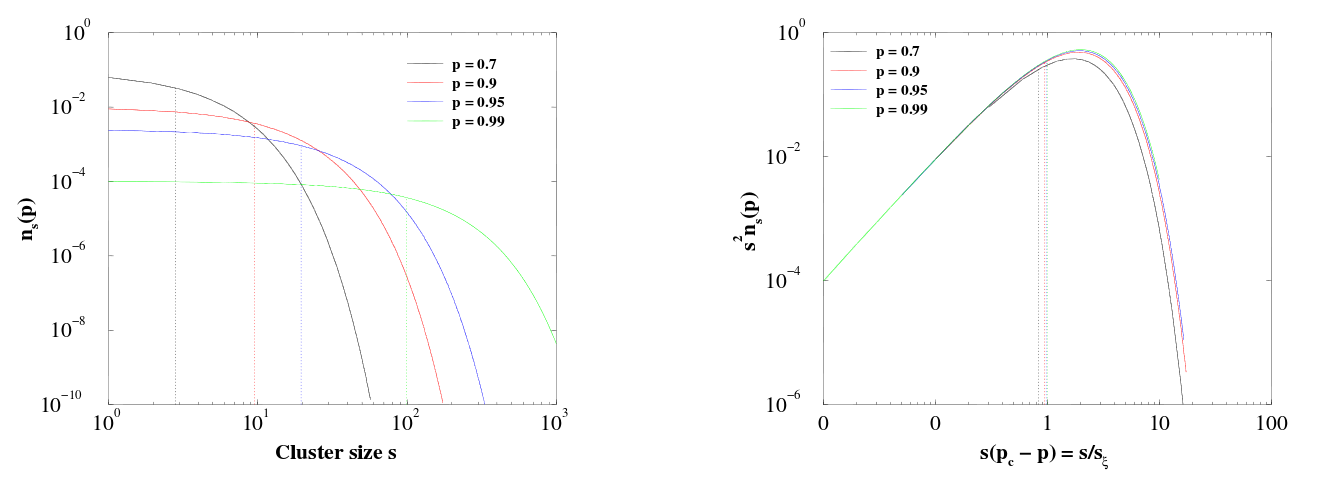
\includegraphics[width=0.8\textwidth]{cluster_num_1d_christensen}
  \caption{Cluster number distribution in 1d.  Dotted vertical lines in both
           figures are the cutoff cluster size $s_\xi$.  In the left figure we note
           power law behavior when $s<s_\xi$ and exponential decay when $s>x_\xi$.
           On the right, we observe that when scaled properly, the distributions 
           collapse onto a single curve as $p\to p_c$.
           Taken from \cite{Christensen2002}.}
  \label{fig:cluster_num_1d}
\end{figure}
This suggests that cluster number distribution scales as a power of $s$
mulitiplied by a function
of the single variable $s/s_\xi = (p-p_c)^{\frac{1}{\sigma}}s$. For 1d
this is apparently $n_s(p) = s^{-2} f(s/s_\xi)$ with $f(x) = x^2 e^{-x}$.
A similar argument for the Bethe lattice suggests the form 
$n_s(p) \propto s^{-5/2} f(s/s_\xi)$ with $f(x) = e^{-x}$.  We would like to
posit the general form $n_s(p) \propto s^{-\tau} f(s/s_\xi)$ but we
encounter a problem in the argument of $f$. From the 
perimeter expansion for $n_s(p)$ we
know $n_s(p)$ is polynomial in $p$ and thus all derivatives are smooth.
However if the argument of the function is of the form $(p-p_c)^{\frac{1}{\sigma}}s$
 with noninteger 
$\frac{1}{\sigma}$, derivatives will generate negative powers of $(p - p_c)$
and thus singularities. To sidestep this difficulty, we modify the argument of
the function $(p-p_c)^{\frac{1}{\sigma}}s \Rightarrow (p-p_c)s^\sigma$
and require that all derivatives of our function are also smooth.

Our final scaling form is thus,
\[n_s(p) \propto s^{-\tau} f((p-p_c)s^\sigma) \]
for large $s$ and $p\to p_c$.  Generally $f(x)$ is slowly varying
for $x \ll 1$ and decays exponentially for $x \gg 1$.  The exponents $\tau$
and $\sigma$ and the function $f$ are independent of the lattice details
and depend only on dimensionality.  In analogy to thermal phase transitions
we may use this relationship to derive scaling laws relating our critical
exponents. For a few examples:
\begin{itemize}
\item The divergence in the average cluster size as $p\to p_c^-$ is driven
by the numerator $\sum_s s^2 n_s(p).$ As this sum diverges due to contributions
at large $s$, we may extract the scaling of the divergence by converting the sum
to an integral,
\begin{align*}
\sum_s s^{2-\tau}f((p-p_c)s^\sigma) \approx& \int^\infty_1 ds\: 
                                          s^{2-\tau}f((p-p_c)s^\sigma) \\
\approx& (p-p_c)^\frac{\tau-3}{\sigma} \int_{(p-p_c)}^\infty
                                    dz \frac{1}{\sigma} |z|^\frac{3-\sigma-\tau}
                                                         {\sigma} f(z).
\end{align*}
As the divergence was at large $s$ we may set the lower limit to 0
and identify \(\gamma = \frac{3-\tau}{\sigma}\).

\item When we attempt to calculate the power, $P = p - \sum_s s n_s(p)$ the
sum is finite and conversion to an integral will not work.  Furthermore, the
difference with p does not allow us to extract the scaling.  We circumvent
this by taking two derivatives with respect to $p$, yielding the relation,
\begin{align*}
(p-p_c)^{\beta-2} \propto& \int^\infty_1 ds\: 
                                          s^{1-\tau + 2\sigma}f((p-p_c)s^\sigma) \\
\approx& (p-p_c)^\frac{2-\tau+2\sigma}{\sigma} \int_{(p-p_c)}^\infty
                                    dz \frac{1}{\sigma} |z|^\frac{2-\tau+\sigma}
                                                         {\sigma} f(z).
\end{align*}
Which yields the relation $\beta = \frac{\tau-2}{\sigma}$.

\item We may also define a specific heat exponent in analogy to the scaling
of the free energy in thermal transitions.  The number of finite clusters
per lattice site $M_0 = \sum_s n_s(p) \propto (p-p_c)^{2-\alpha}$.  An
argument similar to the last two yields $2-\alpha = \frac{\tau -1}{\sigma}$.
\end{itemize}
Combining these three relationships to eliminate $\tau$ and $\sigma$ gives
the familiar Rushbrooke scaling law, $\alpha + 2\beta + \gamma = 2$.

%==================================================================================
% RENORMALIZATION
%==================================================================================

\section{Renormalization}

The percolation problem is in some ways a more accessible environment in which to
apply renormalization methods.  As we are able to renormalize the probabilites
directly and in real space, the procedure is simplified and thus more conceptually
clear. To avoid a digression into a mapping to the Potts model in order
to apply momentum space RG, only real-space methods will be discussed here.
 As the lattice tranformation in site percolation is somewhat more
transparent, we will walk through the RG steps using it as an example.
\begin{enumerate}
\item[I] We begin by replacing the lattice with a 'superlattice' of
blocks of linear size $l$.  As in thermal transitions, the new lattice
should carry the same symmetry as the old such that renormalization may
be repeated.

On the triangular lattice in site percolation, we may
select triangle of three sites which will become a single site on the
'superlattice.'  This gives a linear size of $l=\sqrt{3}$.

\item[II] Blocks in the old lattice are averaged to determine a new
probability $p' = R_l(p)$.

The RG will shift the probability of our latticeWe use a majority rule to determine the state of the 'superblock.' The
probability that two or more sites are occupied is,
\[p' = R_l(p) = p^3 + 3p^2(1-p) = 3p^2 - 2p^3.\]
This gives the fixed points $R_l(p^*) = p^* = 0, 1, \frac{1}{2}$.

\item[III] We restore the original lattice dimensions by rescaling by $l$.

The correlation length in our new model is $\xi' = \frac{\xi}{l}$.
Near the percolation threshold we have 
$|R_l(p) - p_c|^{-\nu} = \frac{|p-p_c|^{-\nu}}{l}$.
A bit of rearrangement yields a formula for $\nu$,
\[\nu = \frac{\log(l)}{\log\left[\frac{|R_l(p) - R_l(p_c)|}{|p-p_c|}\right]} =
\frac{\log(l)}{\log\left[\left.\d{R_l(p)}{p}\right|_{p^*}\right]}\]

Evaluating this on the triangular lattice gives
\[\nu = \frac{\log(\sqrt{3})}{\log(3/2)} = 1.355\]
which when compared to the exact values of $p_c = \frac{1}{2}$ and
$\nu = \frac{4}{3}$ is quite impressive for the investment.
\end{enumerate}

For bond percolation, we are required to choose a slightly more complicated
transformation.  We consider the square lattice in 2 dimensions and choose
a $2x2$ block of bonds to renormalize upon (see figure FIGURE).  Bonds along the bottom and right sides
of the block are left to neighboring blocks and the block will be replaced by
two bonds, one along the top and another along the left side which will be
placed with a probability $p'$ in the superlattice.  The cluster spanning rule
stipulates that the horizontal superbond will be occupied if the original
block percolates from left to right, and the vertical superbond will be placed
if it percolates vertically.  The symmetry of the block requires that these
two events occur with equal probability and we thus only consider
horizontal percolation.  The possible percolating pond structures are displayed
in figure FIGURE.  These give the RG transformation,
\[R_2(p) = 2p^5 - 5p^4 + 2p^3 + 2p^2\]
with the fixed points,
\[R_2(p^*) = p^* = 0, 1, \frac{1}{2}.\]
The RG approximation for bond percolation on the square lattice thus gives
the exact percolation threshold $p_c = \frac{1}{2}$ and approximate 
critical exponent $\nu = \frac{\log(2)}{\log(\frac{13}{8})} = 1.428$ for
the exact value $\nu=\frac{4}{3}$.

\section{Extensions}
\bibliography{percolation}
\end{document}
